\documentclass{article}
\usepackage{graphicx}
\usepackage{wrapfig}
\usepackage{amsmath}
\usepackage{verbatim}
\usepackage{makeidx}
\usepackage{float}
\usepackage{subfig}
\usepackage[left=1in,top=1in,right=1in]{geometry}

\title{Simulating the Mobot and Linkbot}  
\author{Kevin Gucwa\\Mechanical and Aerospace Engineering}
\date{\today} 
\makeindex

\begin{document}

\begin{center}
{\Huge\sf\bf RoboSim User's Guide}\\
\vspace*{2.5cm}
{\Large\bf Version 0.5.0}
\vspace{4.5cm}
\end{center}

%\maketitle
\newpage
\tableofcontents
\newpage

\section{Introduction}
\texttt{RoboSim} is designed to test programs written to control Barobo Mobot
and Linkbot modules within a simulated environment.  It has been designed to
allow any Ch code which can control hardware Barobo robots to now control them
from within a simulated environment making zero changes to the code.  The
RoboSim GUI allows users to change between hardware and simulated robots and
position the robots in their initial position for simulation.

\section{RoboSim GUI}
\label{sec:gui}
The RoboSim GUI, shown in Figure \ref{fig:gui}, allows users to configure their
computer to run simulated robots in place of the hardware ones.  There is no
save button within the GUI, all changes are automatically saved on each click.

\begin{figure}[H]
	\begin{center}
		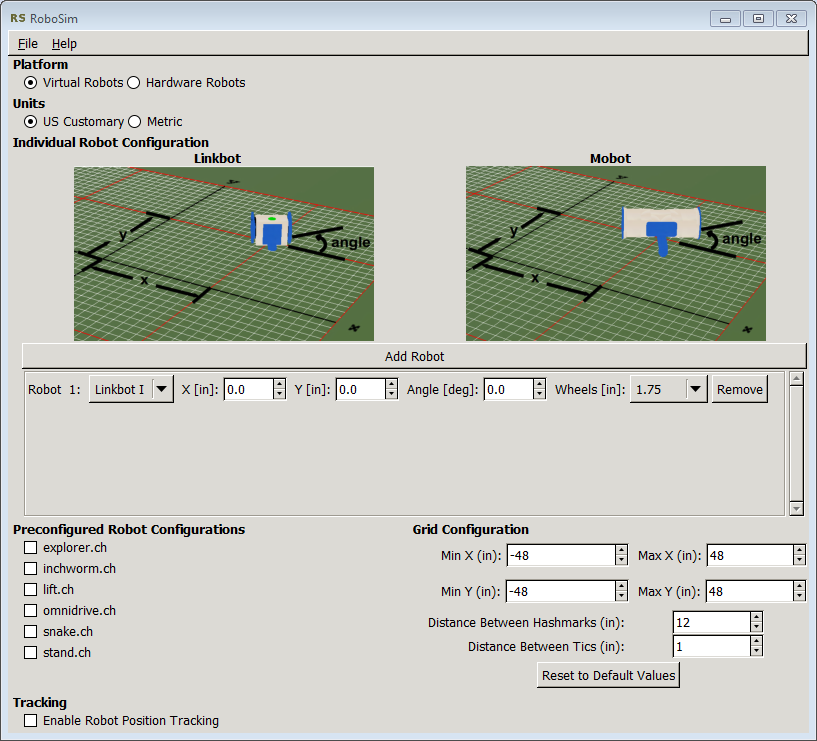
\includegraphics[width=6in]{images/gui}
	\end{center}
	\caption{The RoboSim GUI.}
	\label{fig:gui}
\end{figure}

\subsection{Platform}
This lets a user pick whether the output is sent to the hardware or simulated
robots.  Each time a new Ch code is started, it will check this variable.
Therefore to run subsequent trials on simulated and hardware robots, run the Ch
code with the simulated button checked.  Close the code, change to 'Hardware
Robots' and then rerun the same code.  It will now output to the physical
robots.
\begin{figure}[H]
	\begin{center}
		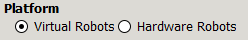
\includegraphics[width=3in]{images/platform}
	\end{center}
	\caption{Initial robot configuration dialog.}
	\label{fig:platform}
\end{figure}

\subsection{Units}
Simulations within RoboSim can be run either in US Customary units consisting of
inches, degrees, and seconds or Metric units with centimeters, degrees, and
seconds.  Changing units will effect the grid spacing drawn beneath the robots
and the spacing between robots.  Changing between these two options will
change the labels within the GUI to indicate the units being used.

\subsection{Individual Robot Configuration}
Initial robot configurations can either be done through the individual robot
section or the preconfigured options.  The individual robot section has options
to allow robots to be positioned within the simulated scene either with or
without wheels but not attached to each other.
\begin{figure}[H]
	\begin{center}
		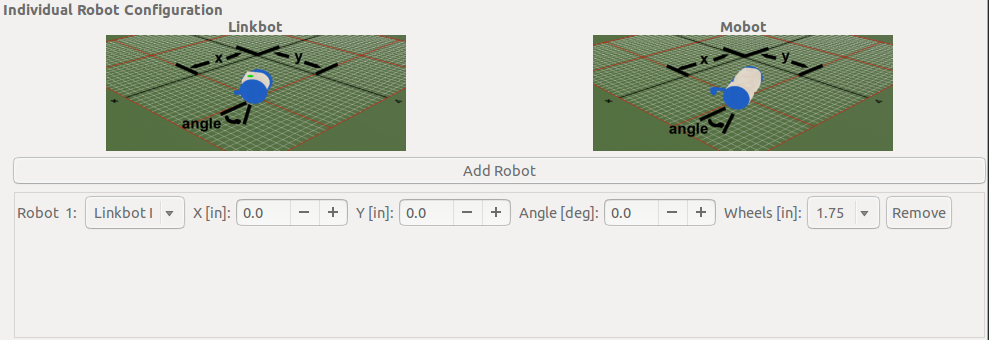
\includegraphics[width=6in]{images/individual}
	\end{center}
	\caption{Individual robot configuration dialog.}
	\label{fig:config}
\end{figure}

Images for the Linkbot and Mobot showing the meaning of each of the options is
shown above the configuration box.  These are screenshots of the simulation
program with the robots positioned at 1 foot in both the x and y dimensions and
at an angle of 30 degrees.  These are the dimensions available to initially position
robots within the simulation.

Initially the individual robot list is empty but can be populated by the large
'add robot' button below the configuration images.  Clicking this button will
add more and more robots into the scene each offset from the previous in the
x-direction by 6 inches or 15 centimeters depending upon the units selected.
The order within the robot list will be the order in which the robots will be
read into the simulation program.

\subsubsection{Robot Type}
There are three options for robot type available.  Linkbot-I, Linkbot-L,
and Mobot.  The options are presented in a drop down menu as shown in
Figure \ref{fig:type}.
\begin{figure}[H]
	\begin{center}
		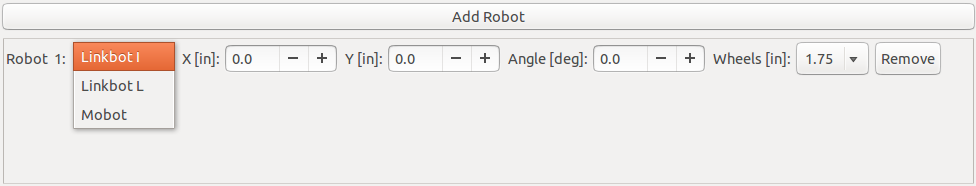
\includegraphics[width=6in]{images/type}
	\end{center}
	\caption{Picking a robot type.}
	\label{fig:type}
\end{figure}

\subsubsection{Robot Position}
Both x and y positions can be chosen independently for each robot.

\subsubsection{Robot Angle}
The rotation angle from the x-axis can be used for changing the orientation of
the two robots respective to each other. 

\subsubsection{Wheels}
Since so many times the robots are run with wheels and a caster connected, a
drop down menu is provided to select different wheel sizes.  The options listed
are the radii of the wheels provided with Linkbots when purchased from Barobo.

\subsubsection{Remove}
Each robot can be removed from the scene by clicking the remove button.  All
remaining robots will remain within the simulation and be at the same positions.

\subsection{Preconfigured Robot Configurations}
In addition to positioning robots independently within the scene, six 
preconfigured options are available to users which represent common Linkbot
configurations.  Selecting one of the options will display a picture of the
configuration built with the hardware Linkbots and corresponding to code within
the C-STEM Learn Linkbot book.  When one of these options is selected, the
specific configuration for this setup is passed into Ch and any robots in the
individual robot list are ignored.  To switch back to the individual
configuration, just unselect the selected robot configuration.
\begin{figure}[H]
	\begin{center}
		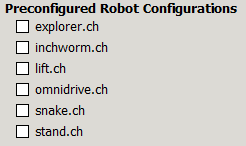
\includegraphics[width=4in]{images/preconfig}
	\end{center}
	\caption{Preconfigured Linkbots.}
	\label{fig:preconfig}
\end{figure}

\subsection{Grid Configuration}
To be able to see how far robots have moved, a grid is enabled under the robots.
There are three options to alter the layout of the grid lines.  Total distance
is the entire distance between -x and x for which grid lines will be displayed.
Hashmarks are the red lines drawn within the configuration images.  By default
they are every foot.  Tics are the most frequent lines drawn in a light gray
and by default every inch.  Switching between US Customary and Metric units will
change these default values to logical starting points for the metric system.

\subsection{Tracking}
Tracking where robots have been can be enabled by default by selecting the
check box.  This will draw green lines which draw out everywhere that each robot
has been.  Once a simulation is running, the tracking line can be enabled or
disabled by pressing the 't' key.

\section{Running a Simulation}
Once the simulation environment has been configured with the RoboSim GUI in
Section \ref{sec:gui}, users can now run code written to control the hardware
Barobo robots within simulation.  The RoboSim GUI should remain open while
simulating robots, once it is closed, it will revert to hardware mode.  The
graphics for each simulation are created upon running the code.

\section{Interacting with a Simulation}
The simulation window responds to mouse inputs to allow users to move about the
scene.  The mouse wheel or right mouse button allows zooming in and out from the
robots.  Holding the left button rotates the camera about the viewpoint.
Clicking, holding, and dragging both mouse buttons pans around the scene to
change the camera location.

The ground plane is for reference only.  It is designed to disappear when
viewing the robots from below to be able to inspect the movement from all
angles.

\subsection{Keyboard Input}
The simulation will respond to keyboad input as outlined in Table
\ref{tab:keys}.

\begin{table}[H]
	\begin{center}
	\begin{tabular}{c | l }
		\hline \hline
		\textbf{key} & \textbf{action} \\ \hline
		r & toggle robot visibility and enable tracking \\
		t & toggle robot tracking \\
		any other key & Pause and unpause simulation \\
		\hline \hline
	\end{tabular}
	\caption{Keyboard input for RoboSim}
	\label{tab:keys}
	\end{center}
\end{table}

\subsection{Mouse Input}
The mouse can be used to move the camera around the scene.  Left clicking and
dragging the mouse pans the camera.  Right clicking enables scaling of the view.
Clicking both left and right mouse buttons and dragging changes the location of
the camera within the scene.

Clicking on any robot will enable a pop up which displays the robot name and the
current position of the robot.  Clicking again will disable the display.

\appendix
\section{Manual Configuration File Generation}
\subsection{Robot Attributes}
Each robot element is required to have one attribute titled \textbf{id} which is
an unique identifier for the simulation to reference.  A second optional
attribute is \textbf{orientation} which orients the face of a second robot when
it is being attached to a first robot.

\begin{table}[H]
	\begin{center}
	\begin{tabular}{c | l}
		\hline 
		\verb|<linkboti id="0"/>| & one linkbot I with id = 0 \\
		\verb|<linkboti id="0" orientation="3"/>| & Linkbot I is 'upside-down' \\
		\hline
	\end{tabular}
	\caption{Examples}
	\label{tab:ex}
	\end{center}
\end{table}

\begin{table}[H]
	\begin{center}
	\begin{tabular}{c | c | l}
		\hline \hline
		\textbf{attribute} & \textbf{values} & \textbf{description} \\ \hline
		id & unique integer & a unique integer to identify each robot \\
		orientation & 1 & robot face number is at 12 o'clock \\
		 & 2 & robot face number is at 3 o'clock \\
		 & 3 & robot face number is at 6 o'clock \\
		 & 4 & robot face number is at 9 o'clock \\
		\hline \hline
	\end{tabular}
	\caption{Robot Attributes}
	\label{tab:attributes}
	\end{center}
\end{table}

\end{document}
